135. \begin{figure}[ht!]
\center{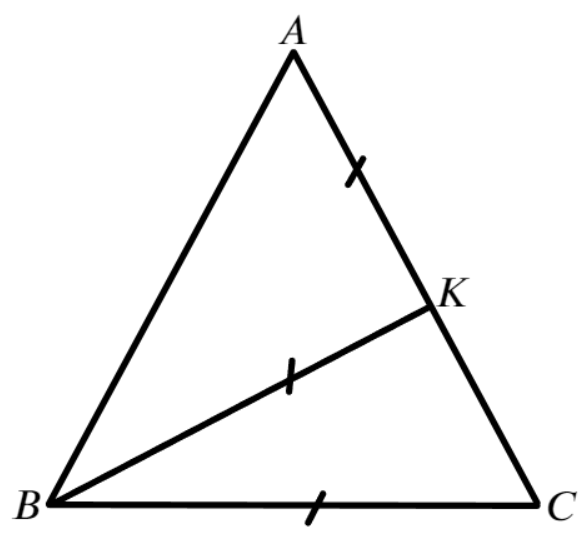
\includegraphics[scale=0.35]{g7-135.png}}
\end{figure}\\
Пусть $CB=BK=KA=x,$ а $KC=y,$ тогда $AB=AC=x+y$ и имеет место система уравнений $\begin{cases} 2x+y=6,\\ 3x+y=7.\end{cases}$ откуда $x=1,\ y=4.$ Но тогда в треугольнике $BKC$ получаем $BK+BC=1+1=2<4=CK,$ что невозможно по неравенству треугольника. Значит, такого треугольника не существует.\\
